\chapter{Entrada de dados}

Agora ser\'a apresentado como capturar dados a partir da entrada padr\~ao e armazenar seu conte\'udo em uma vari\'avel.

\begin{figure}[!htb]
	\centering
	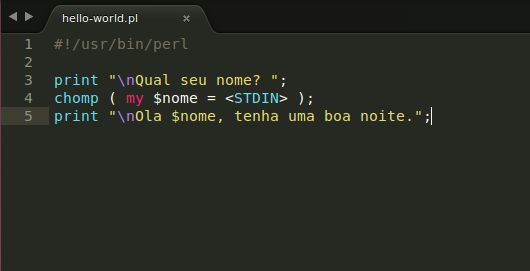
\includegraphics[width=0.5\textwidth]{../5_figuras/image7}
	\caption{Algoritmo com captura da entrada padr\~ao}
\end{figure}

Na figura 7, linha 4 a vari\'avel \$nome que recebe o valor de \textit{$<$STDIN$>$}, que \'e a fun\c{c}\~ao que l\^e uma linha da entrada padr\~ao, 
nesse caso, o teclado. O que \'e chomp? \'E a fun\c{c}\~ao que elimina o \'ultimo caractere caso esse \'ultimo caractere seja um o comando de escape 
respons\'avel pela quebra da linha (\textbackslash n). A sa\'ida do algoritmo segue na figura 8.

\begin{figure}[!htb]
	\centering
	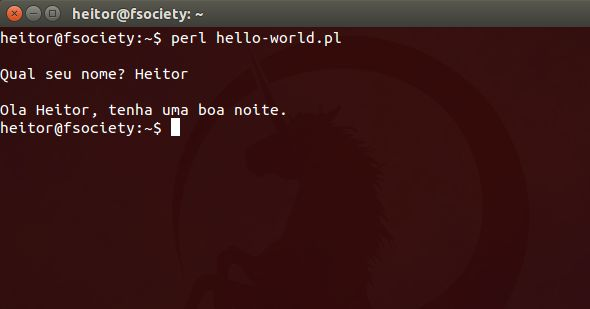
\includegraphics[width=0.5\textwidth]{../5_figuras/image8}
	\caption{Sa\'ida do algoritmo de captura da entrada padr\~ao}
\end{figure}

Hora de colocar o conhecimento adquirido em pr\'atica. 

\begin{figure}[!htb]
	\centering
	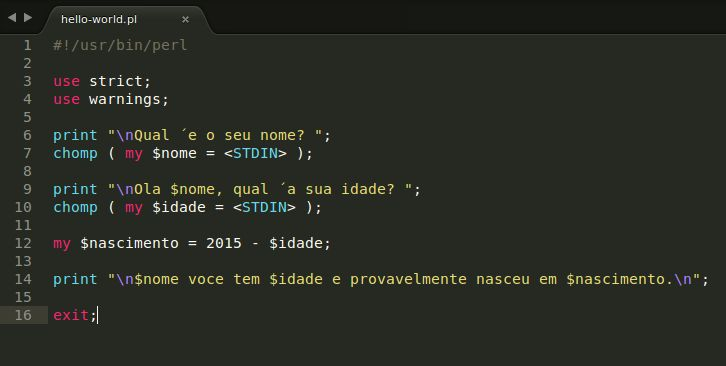
\includegraphics[width=0.5\textwidth]{../5_figuras/image9}
	\caption{Modelo de algoritmo a se adotar}
\end{figure}

Bom, a seguir \'e apresentado algumas alguns conceitos novos. O primeiro \'e o conceito de m\'odulos; m\'odulos s\~ao bibliotecas que mudam o modo de 
interpreta\c{c}\~ao do Perl. Na figura 9, na 3$^a$ e 4$^a$ linha s\~ao usados os m\'odulos \textit{strict} e \textit{warnings}. O \textit{use} 
indica ao interpretador quais m\'odulos a serem ativados.

\textit{strict} e \textit{warnings} ajuda a evitar os principais erros e enganos comuns nos c\'odigos em perl, por isso s\~ao extremamente \'uteis e 
recomenda-se o seu uso. 
  
Na linha 12 \'e efetuada uma opera\c{c}\~ao m\'atematica simples para descobrir o ano de nascimento do usu\'ario a partir na idade informada, a l\'ogica
para resolver esse problema \'e basicamente a idade menos o ano informado que retornar\'a o ano de nascimento. Depois \'e feita uma chamada de \textit{print}
para escrita na sa\'ida padr\~ao de dados. A sa\'ida \'e apresentada na figura 10.

\begin{figure}[!htb]
	\centering
	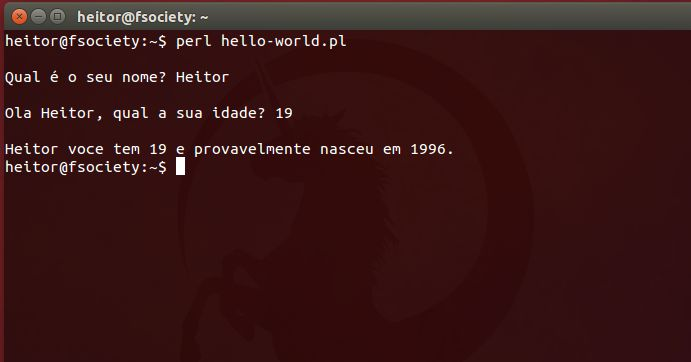
\includegraphics[width=0.5\textwidth]{../5_figuras/image10}
	\caption{Sa\'ida do algoritmo}
\end{figure}